\documentclass[11pt]{article}
\usepackage[textwidth=18.0cm, textheight=23.0cm, top=2.0cm]{geometry}
\usepackage{pst-all}
\usepackage{amssymb}
\usepackage{tikz}
\usepackage{underscore}\begin{document}
\pagestyle{empty}


ClassName: \underline{\textbf{Class_10.2bp-11}}
\par
BinSize: \underline{\textbf{100 × 100}}
\par
ReduceSize: \underline{\textbf{100 × 100}}
\par
TypeNum: \underline{\textbf{40}}
\par
Num: \underline{\textbf{40}}
\par
OutS: \underline{\textbf{80000}}
\par
InS: \underline{\textbf{66055}}
\par
Rate: \underline{\textbf{0.826}}
\par
UB: \underline{\textbf{8}}
\par
LB0: \underline{\textbf{7}}
\par
LB: \underline{\textbf{8}}
\par
LBWithCut: \underline{\textbf{8}}
\par
NodeCut: \underline{\textbf{0}}
\par
ExtendedNodeCnt: \underline{\textbf{1}}
\par
GenNodeCnt: \underline{\textbf{1}}
\par
PrimalNode: \underline{\textbf{0}}
\par
ColumnCount: \underline{\textbf{34}}
\par
TotalCutCount: \underline{\textbf{0}}
\par
RootCutCount: \underline{\textbf{0}}
\par
LPSolverCnt: \underline{\textbf{27}}
\par
PricingSolverCnt: \underline{\textbf{27}}
\par
BranchAndBoundNum: \underline{\textbf{1}}
\par
isOpt: \underline{\textbf{false}}
\par
TimeOnInitSolution: \underline{\textbf{600.000 s}}
\par
TimeOnPrimal: \underline{\textbf{0.000 s}}
\par
TimeOnPricing: \underline{\textbf{2999.617 s}}
\par
TimeOnRmp: \underline{\textbf{0.093 s}}
\par
TotalTime: \underline{\textbf{3599.992 s}}
\par
\newpage


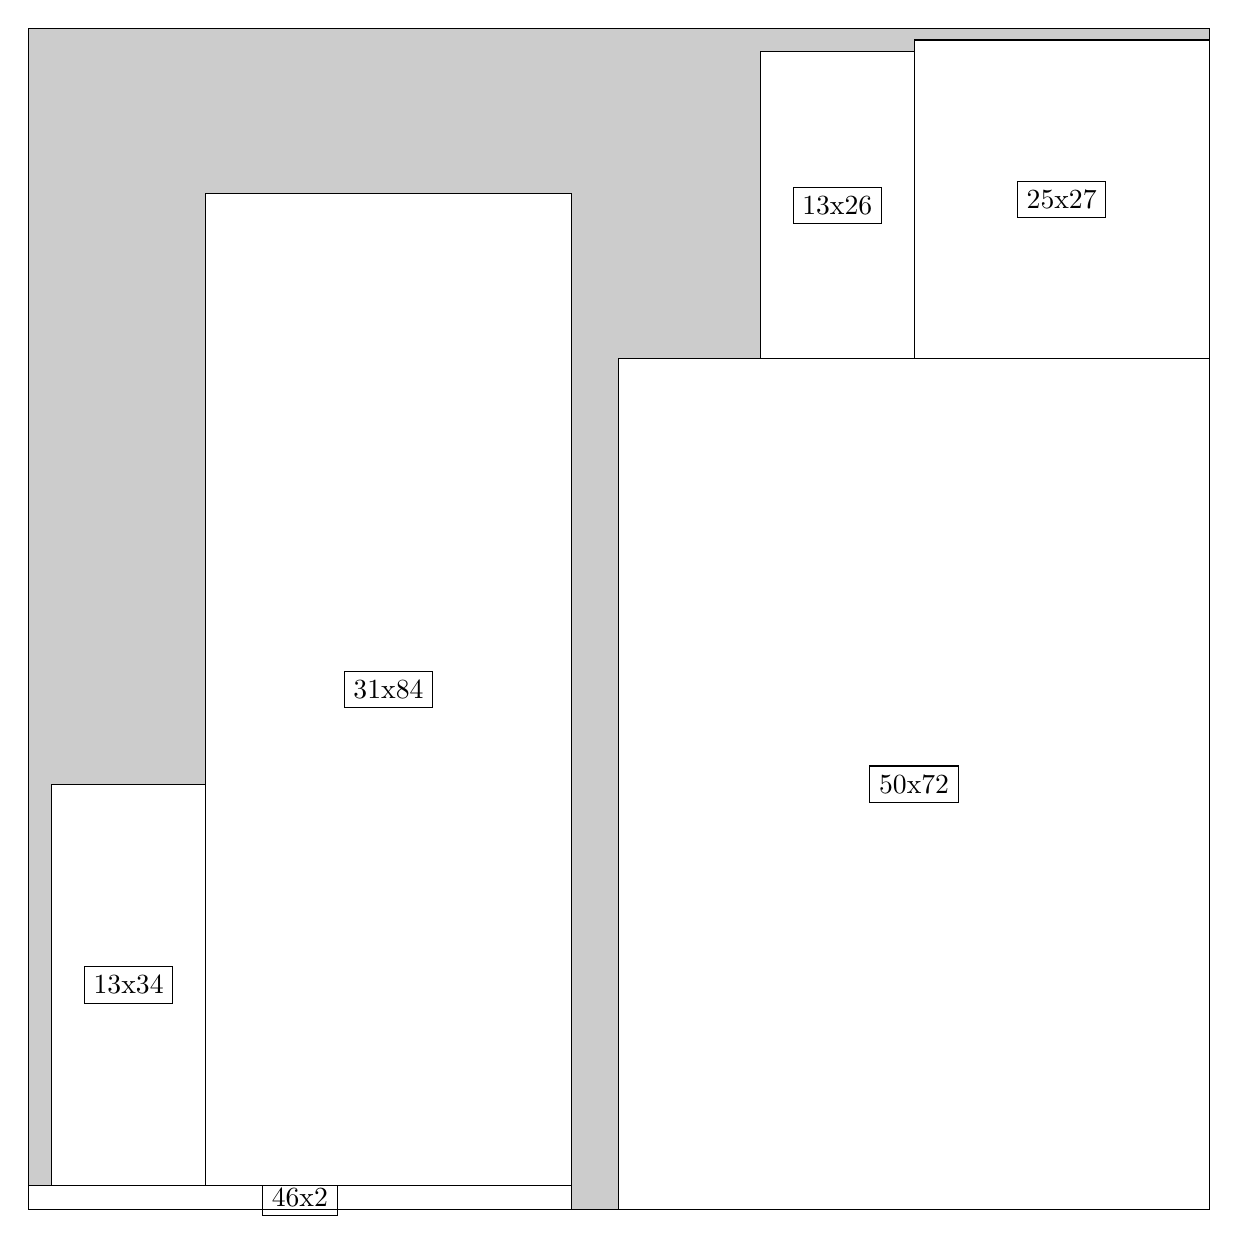
\begin{tikzpicture}[shorten >=1pt,scale=1.0,every node/.style={scale=1.0},->]
\tikzstyle{vertex}=[circle,fill=black!25,minimum size=14pt,inner sep=0pt]
\filldraw[fill=gray!40!white, draw=black] (0,0) rectangle (15.0,15.0);
\foreach \name/\x/\y/\w/\h in {50x72/7.5/0.0/7.5/10.799999999999999,25x27/11.25/10.799999999999999/3.75/4.05,13x26/9.299999999999999/10.799999999999999/1.95/3.9,46x2/0.0/0.0/6.8999999999999995/0.3,31x84/2.25/0.3/4.6499999999999995/12.6,13x34/0.3/0.3/1.95/5.1}
\filldraw[fill=white!40!white, draw=black] (\x,\y) rectangle node[draw] (\name) {\name} ++(\w,\h);
\end{tikzpicture}


w =50 , h =72 , x =50 , y =0 , v =3600
\par
w =25 , h =27 , x =75 , y =72 , v =675
\par
w =13 , h =26 , x =62 , y =72 , v =338
\par
w =46 , h =2 , x =0 , y =0 , v =92
\par
w =31 , h =84 , x =15 , y =2 , v =2604
\par
w =13 , h =34 , x =2 , y =2 , v =442
\par
\newpage


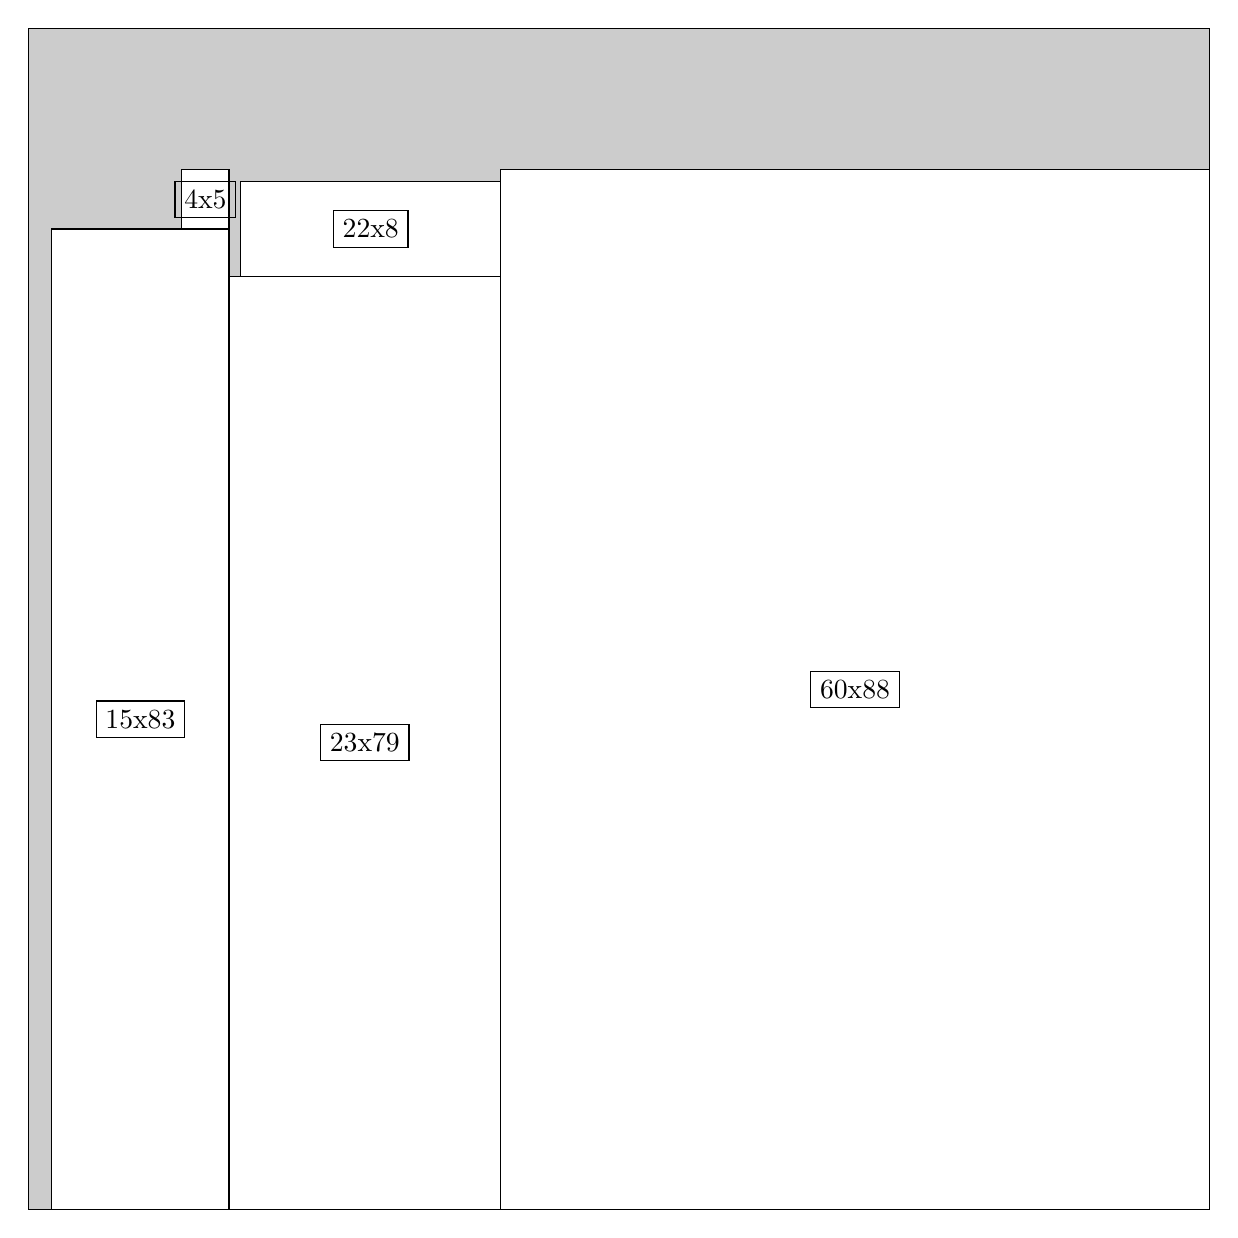
\begin{tikzpicture}[shorten >=1pt,scale=1.0,every node/.style={scale=1.0},->]
\tikzstyle{vertex}=[circle,fill=black!25,minimum size=14pt,inner sep=0pt]
\filldraw[fill=gray!40!white, draw=black] (0,0) rectangle (15.0,15.0);
\foreach \name/\x/\y/\w/\h in {60x88/6.0/0.0/9.0/13.2,23x79/2.55/0.0/3.4499999999999997/11.85,22x8/2.6999999999999997/11.85/3.3/1.2,15x83/0.3/0.0/2.25/12.45,4x5/1.95/12.45/0.6/0.75}
\filldraw[fill=white!40!white, draw=black] (\x,\y) rectangle node[draw] (\name) {\name} ++(\w,\h);
\end{tikzpicture}


w =60 , h =88 , x =40 , y =0 , v =5280
\par
w =23 , h =79 , x =17 , y =0 , v =1817
\par
w =22 , h =8 , x =18 , y =79 , v =176
\par
w =15 , h =83 , x =2 , y =0 , v =1245
\par
w =4 , h =5 , x =13 , y =83 , v =20
\par
\newpage


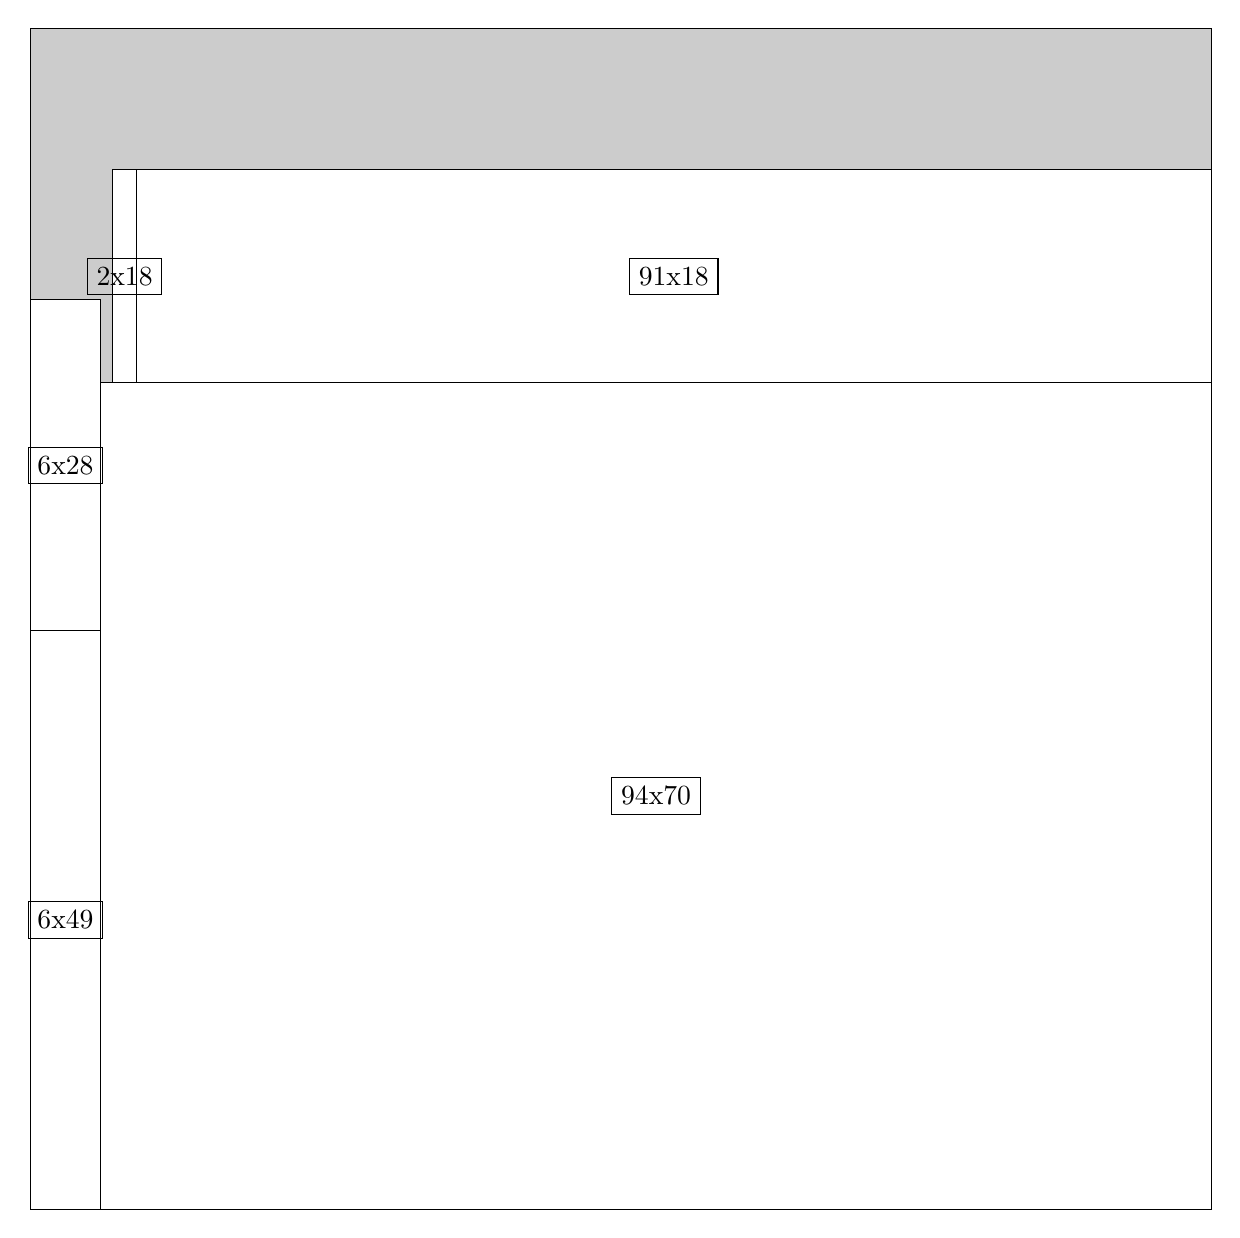
\begin{tikzpicture}[shorten >=1pt,scale=1.0,every node/.style={scale=1.0},->]
\tikzstyle{vertex}=[circle,fill=black!25,minimum size=14pt,inner sep=0pt]
\filldraw[fill=gray!40!white, draw=black] (0,0) rectangle (15.0,15.0);
\foreach \name/\x/\y/\w/\h in {94x70/0.8999999999999999/0.0/14.1/10.5,91x18/1.3499999999999999/10.5/13.65/2.6999999999999997,2x18/1.05/10.5/0.3/2.6999999999999997,6x49/0.0/0.0/0.8999999999999999/7.35,6x28/0.0/7.35/0.8999999999999999/4.2}
\filldraw[fill=white!40!white, draw=black] (\x,\y) rectangle node[draw] (\name) {\name} ++(\w,\h);
\end{tikzpicture}


w =94 , h =70 , x =6 , y =0 , v =6580
\par
w =91 , h =18 , x =9 , y =70 , v =1638
\par
w =2 , h =18 , x =7 , y =70 , v =36
\par
w =6 , h =49 , x =0 , y =0 , v =294
\par
w =6 , h =28 , x =0 , y =49 , v =168
\par
\newpage


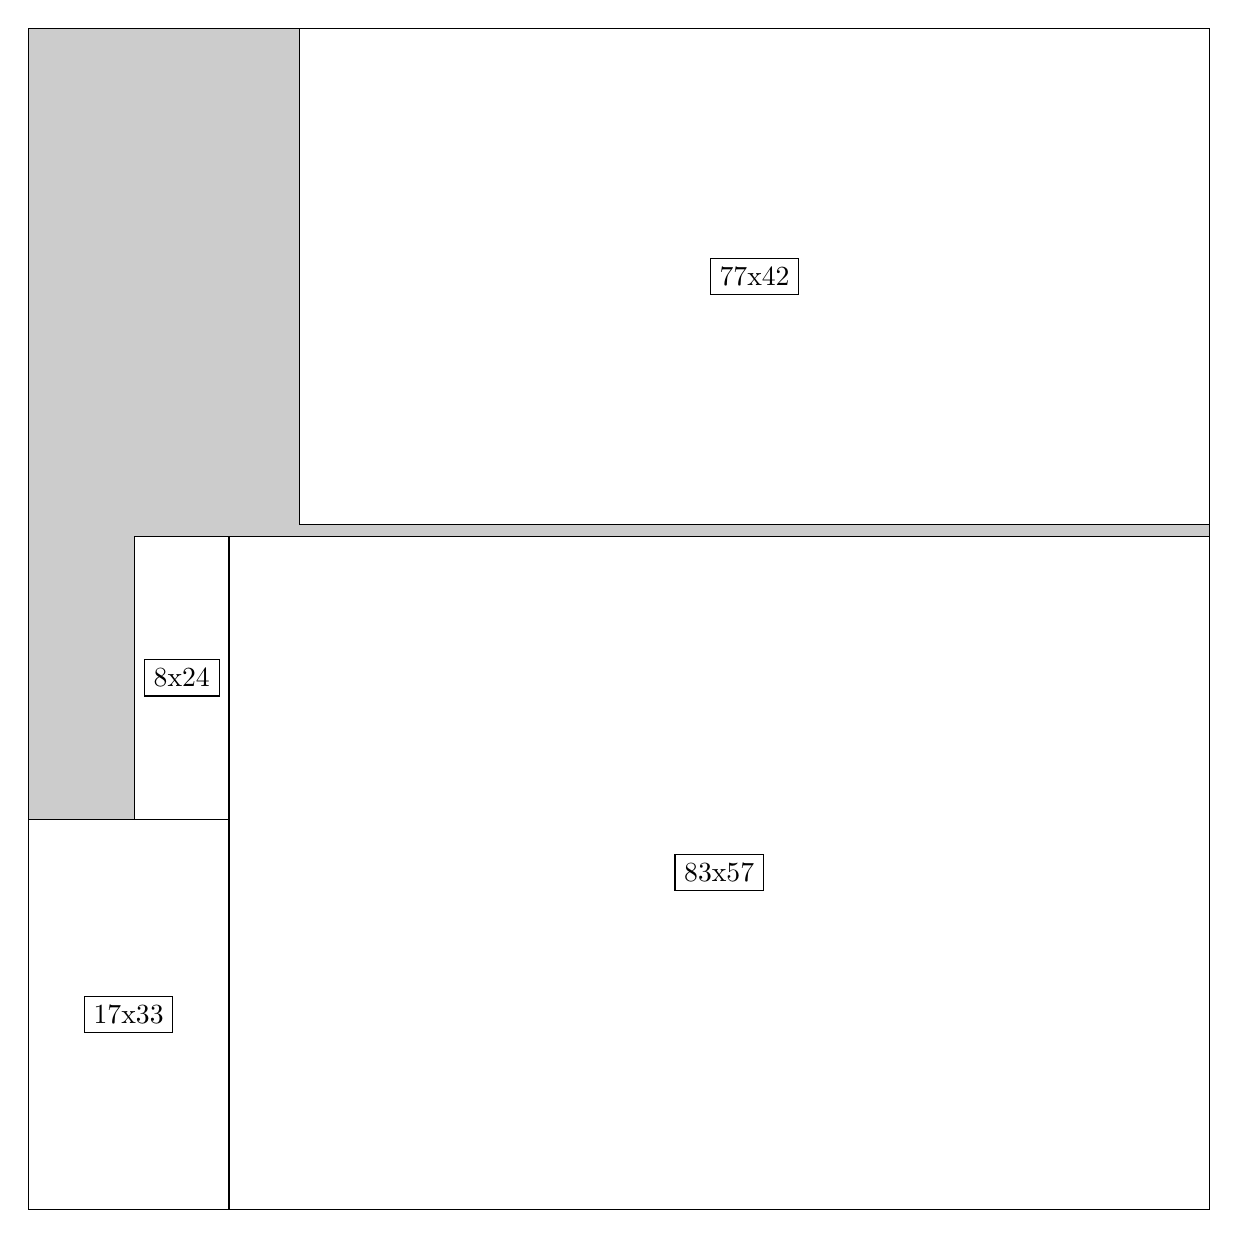
\begin{tikzpicture}[shorten >=1pt,scale=1.0,every node/.style={scale=1.0},->]
\tikzstyle{vertex}=[circle,fill=black!25,minimum size=14pt,inner sep=0pt]
\filldraw[fill=gray!40!white, draw=black] (0,0) rectangle (15.0,15.0);
\foreach \name/\x/\y/\w/\h in {83x57/2.55/0.0/12.45/8.549999999999999,17x33/0.0/0.0/2.55/4.95,8x24/1.3499999999999999/4.95/1.2/3.5999999999999996,77x42/3.4499999999999997/8.7/11.549999999999999/6.3}
\filldraw[fill=white!40!white, draw=black] (\x,\y) rectangle node[draw] (\name) {\name} ++(\w,\h);
\end{tikzpicture}


w =83 , h =57 , x =17 , y =0 , v =4731
\par
w =17 , h =33 , x =0 , y =0 , v =561
\par
w =8 , h =24 , x =9 , y =33 , v =192
\par
w =77 , h =42 , x =23 , y =58 , v =3234
\par
\newpage


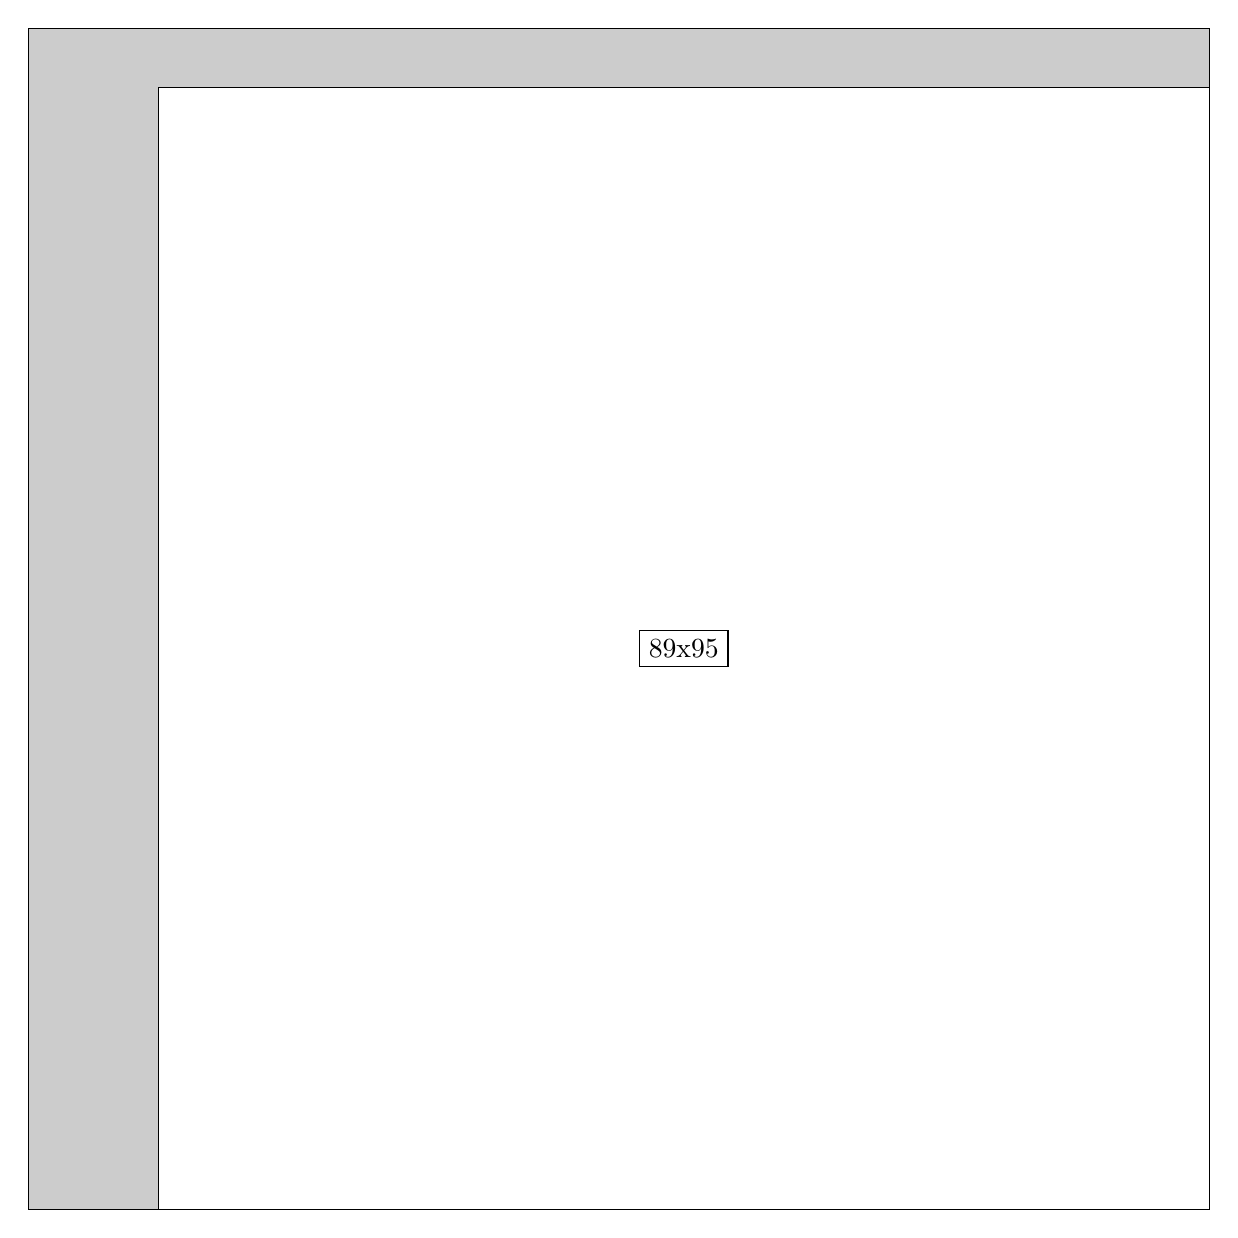
\begin{tikzpicture}[shorten >=1pt,scale=1.0,every node/.style={scale=1.0},->]
\tikzstyle{vertex}=[circle,fill=black!25,minimum size=14pt,inner sep=0pt]
\filldraw[fill=gray!40!white, draw=black] (0,0) rectangle (15.0,15.0);
\foreach \name/\x/\y/\w/\h in {89x95/1.65/0.0/13.35/14.25}
\filldraw[fill=white!40!white, draw=black] (\x,\y) rectangle node[draw] (\name) {\name} ++(\w,\h);
\end{tikzpicture}


w =89 , h =95 , x =11 , y =0 , v =8455
\par
\newpage


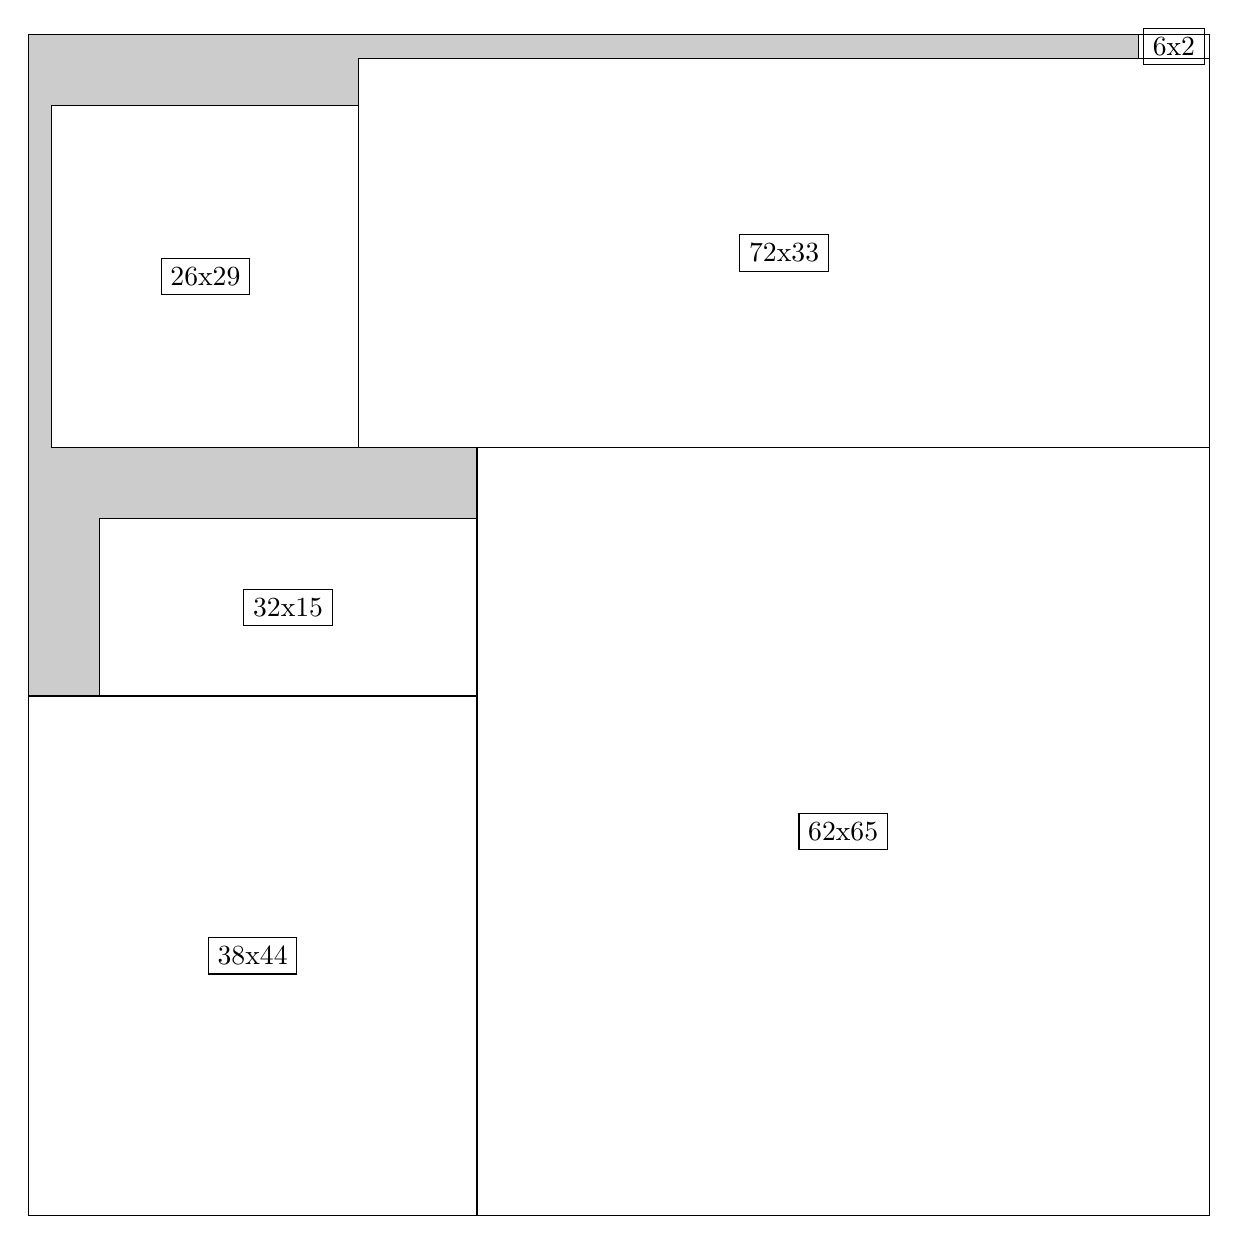
\begin{tikzpicture}[shorten >=1pt,scale=1.0,every node/.style={scale=1.0},->]
\tikzstyle{vertex}=[circle,fill=black!25,minimum size=14pt,inner sep=0pt]
\filldraw[fill=gray!40!white, draw=black] (0,0) rectangle (15.0,15.0);
\foreach \name/\x/\y/\w/\h in {62x65/5.7/0.0/9.299999999999999/9.75,38x44/0.0/0.0/5.7/6.6,32x15/0.8999999999999999/6.6/4.8/2.25,72x33/4.2/9.75/10.799999999999999/4.95,6x2/14.1/14.7/0.8999999999999999/0.3,26x29/0.3/9.75/3.9/4.35}
\filldraw[fill=white!40!white, draw=black] (\x,\y) rectangle node[draw] (\name) {\name} ++(\w,\h);
\end{tikzpicture}


w =62 , h =65 , x =38 , y =0 , v =4030
\par
w =38 , h =44 , x =0 , y =0 , v =1672
\par
w =32 , h =15 , x =6 , y =44 , v =480
\par
w =72 , h =33 , x =28 , y =65 , v =2376
\par
w =6 , h =2 , x =94 , y =98 , v =12
\par
w =26 , h =29 , x =2 , y =65 , v =754
\par
\newpage


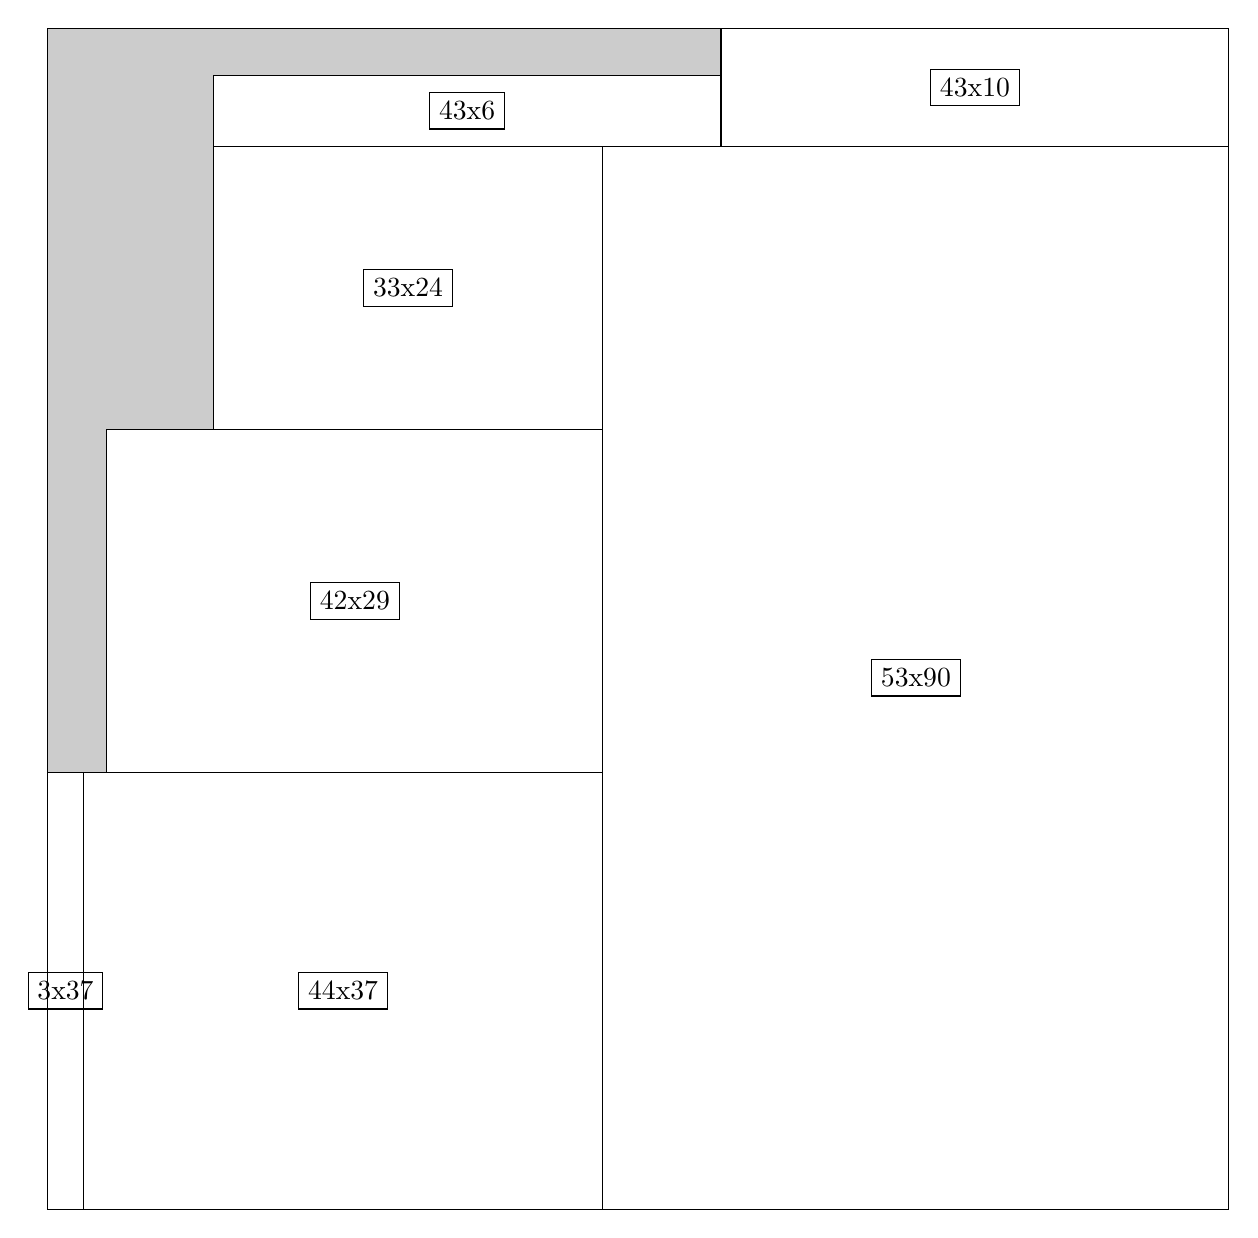
\begin{tikzpicture}[shorten >=1pt,scale=1.0,every node/.style={scale=1.0},->]
\tikzstyle{vertex}=[circle,fill=black!25,minimum size=14pt,inner sep=0pt]
\filldraw[fill=gray!40!white, draw=black] (0,0) rectangle (15.0,15.0);
\foreach \name/\x/\y/\w/\h in {53x90/7.05/0.0/7.949999999999999/13.5,44x37/0.44999999999999996/0.0/6.6/5.55,3x37/0.0/0.0/0.44999999999999996/5.55,42x29/0.75/5.55/6.3/4.35,33x24/2.1/9.9/4.95/3.5999999999999996,43x10/8.549999999999999/13.5/6.45/1.5,43x6/2.1/13.5/6.45/0.8999999999999999}
\filldraw[fill=white!40!white, draw=black] (\x,\y) rectangle node[draw] (\name) {\name} ++(\w,\h);
\end{tikzpicture}


w =53 , h =90 , x =47 , y =0 , v =4770
\par
w =44 , h =37 , x =3 , y =0 , v =1628
\par
w =3 , h =37 , x =0 , y =0 , v =111
\par
w =42 , h =29 , x =5 , y =37 , v =1218
\par
w =33 , h =24 , x =14 , y =66 , v =792
\par
w =43 , h =10 , x =57 , y =90 , v =430
\par
w =43 , h =6 , x =14 , y =90 , v =258
\par
\newpage


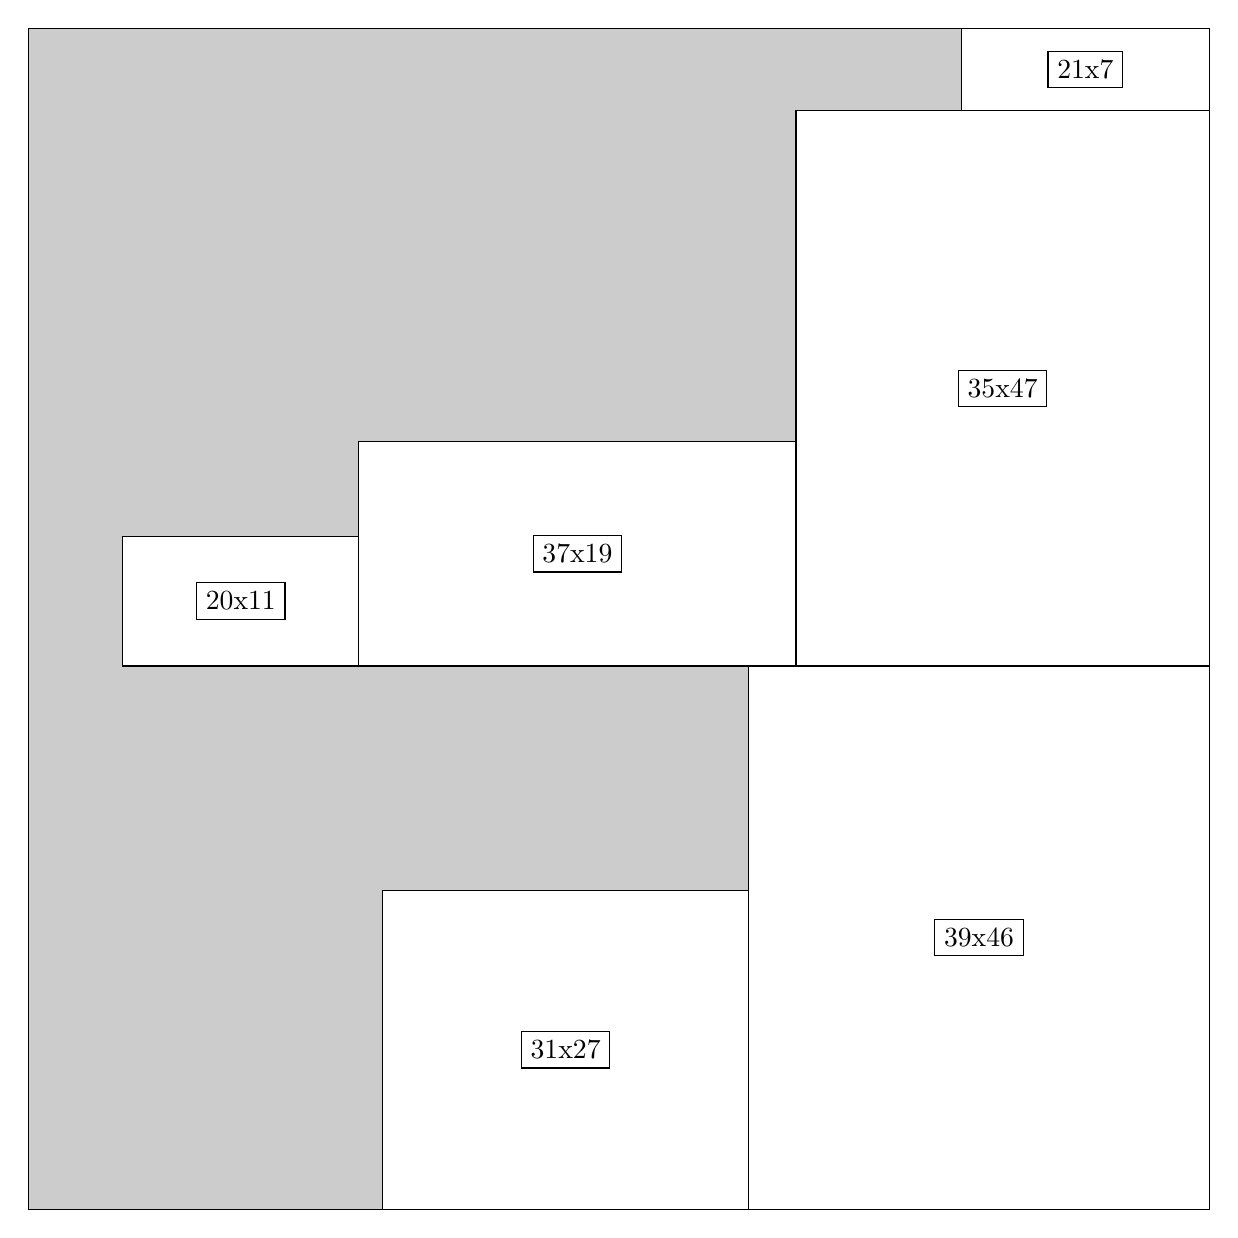
\begin{tikzpicture}[shorten >=1pt,scale=1.0,every node/.style={scale=1.0},->]
\tikzstyle{vertex}=[circle,fill=black!25,minimum size=14pt,inner sep=0pt]
\filldraw[fill=gray!40!white, draw=black] (0,0) rectangle (15.0,15.0);
\foreach \name/\x/\y/\w/\h in {39x46/9.15/0.0/5.85/6.8999999999999995,31x27/4.5/0.0/4.6499999999999995/4.05,35x47/9.75/6.8999999999999995/5.25/7.05,21x7/11.85/13.95/3.15/1.05,37x19/4.2/6.8999999999999995/5.55/2.85,20x11/1.2/6.8999999999999995/3.0/1.65}
\filldraw[fill=white!40!white, draw=black] (\x,\y) rectangle node[draw] (\name) {\name} ++(\w,\h);
\end{tikzpicture}


w =39 , h =46 , x =61 , y =0 , v =1794
\par
w =31 , h =27 , x =30 , y =0 , v =837
\par
w =35 , h =47 , x =65 , y =46 , v =1645
\par
w =21 , h =7 , x =79 , y =93 , v =147
\par
w =37 , h =19 , x =28 , y =46 , v =703
\par
w =20 , h =11 , x =8 , y =46 , v =220
\par
\newpage


\end{document}